\chapter{Methodology}

\section{Research Design}
\label{sec:meth:research_design}
This study uses an experimental pipeline development design in which an \gls{llm}-based biomedical information extraction system is developed iteratively against a fixed benchmark corpus before being frozen and evaluated on independently sampled, contemporary biomedical literature. The study consists of four main stages: development of the extraction pipeline against BioRED, selection of a pipeline iteration, evaluation of the chosen iteration, and construction and evaluation of a knowledge graph from the resulting contemporary extractions.

The main methodological idea of this design was the separation between development and evaluation. BioRED served as a basis for training, development, and test splits where this project's iterative pipeline development, made up of a set of Extraction Pipeline Iterations (\glspl{epi}), was conducted solely against the training and development splits. Each \gls{epi}'s prompt design and configuration was based on the previous \gls{epi}'s performance and optional further error analysis -- this approach began with an initial configuration (EPI 001), discussed further in Section~\ref{sec:meth:pipeline_development}, that established a baseline extraction pipeline using generic biomedical extraction instructions without BioRED-specific schema guidance. Pipeline development continued against the BioRED training split until performance plateaued, at which point the \gls{epi} configurations were frozen and no further prompt refinement or schema adjustment was performed. The frozen iterations were then evaluated against the BioRED development split, where their performance was compared with one another and the best performing \gls{epi} was selected. This distinction allows subsequent evaluation to be treated as a measure of the pipeline's performance, rather than further development.

The final \gls{epi} was then evaluated under two distinct stages. The first is benchmark evaluation, which measures the final \gls{epi}'s extraction performance against BiORED's held-out ground truth, establishing its performance within the distribution it was developed on. The second stage was generalisation evaluation, which applies the same pipeline to an independently assembled corpus of contemporary PubMed literature that the pipeline was not iteratively developed on. As the pipeline was not adapted to perform specifically on the contemporary corpus, any significant degradation in performance between them can be attributed to a change in the dataset's literature distribution, rather than to any changes in the pipeline's configuration, allowing benchmark and contemporary corpus performance to be compared. Following extraction and normalisation on the contemporary corpus, the extracted entities and relations were assembled into a \gls{kg}.

\section{Datasets}
\label{sec:meth:datasets}

\subsection{BioRED Benchmark Corpus}
\label{subsec:meth:biored_benchmark_corpus}
The original BioRED corpus, as described in Section~\ref{subsec:lit:biored}, was used as the benchmark corpus for extraction pipeline development and evaluation in this project. The corpus consists of 600 manually annotated PubMed abstracts, assembled and released by the \gls{ncbi} and was obtained directly from the dataset's public GitHub repository. The BioRED-BC8 extension was also considered as it provides a more recent expert-annotated evaluation set: however, the original BioRED corpus was retained as the controlled benchmark as the study separately evaluates generalisation using literature independently retrieved through the PubMed \gls{api}, better reflecting the intended deployment pathway. BioRED-BC8 therefore represents a valuable alternative external evaluation dataset for future work.

The original version of the BioRED dataset divides 600 abstracts into a training split of 400 abstracts, a development split of 100 abstracts, and a test split of 100 abstracts. Each split was used for a distinct role in this study. The training split was used throughout iterative \gls{epi} development, providing the abstracts observed by the \gls{llm} in which all \gls{epi} configurations were developed on, the development split was then used to evaluate all frozen \gls{epi} configurations against one another, and the test spit was used exclusively for the final benchmark evaluation of the best-performing pipeline configuration and played no role in either pipeline development or \gls{epi} selection.

For each abstract, this project used the associated \gls{pmid}, title, and abstract text as the input passed to the extraction pipeline, together with the corresponding gold-standard annotations used as ground truth. These annotations consisted of each entity's type and text span and each relation's type. The following table summarises how each component of the BioRED dataset was used in this study:

\begin{table}[H]
    \centering
    \caption{BioRED Split Summary}
    \label{tab:biored_split_summary}
    \begin{tabularx}{\textwidth}{l Y Y Y}
        \toprule
        BioRED Component & No. of Abstracts & Purpose \\
        \midrule
        Training spit & 400 & EPI development and performance estimate \\
        Development split & 100 & Held-out generalisation check / EPI selection \\
        Test split & 100 & Final benchmark evaluation \\
        \bottomrule
    \end{tabularx}
\end{table}

It should be noted that \gls{epi} refinement was conducted using a fixed 35-abstract subsample of the BioRED training split, with each final \gls{epi} then evaluated across the full 400-abstract training split. Section~\pref \ discusses this methodological decision further.

BioRED's train, development, and test splits were each retrieved from the official BioRED GitHub repository as separate BioC-XML files. This process is discussed in Section~\ref{subsec:meth:data_preparation}.

\subsection{Contemporary Biomedical Corpus}
\label{subsec:meth:contemporary_biomedical_corpus}
An independently-assembled corpus of contemporary biomedical PubMed abstracts was constructed as the external evaluation set used to investigate generalisation to out-of-distribution data, as mentioned in Section~\ref{sec:lit:generalisation_to_contemporary_biomed_lit}. This \gls{cbc} included abstracts from papers published across 2024, 2025, and 2026 making up 282 total abstracts after duplication removal by \gls{pmid} and removal of entries with missing abstract texts. It should be explicitly noted that this corpus was assembled entirely independently of BioRED and played no role in \gls{epi} development or selection.

"Contemporary biomedical literature" was defined through a fixed set of either PubMed research queries, designed to give broad coverage of the wider field of general biomedicine, rather than a single subdomain. Four of the eight related to individual biomedical entity categories, generally mirroring BioRED's own entity type (gene/protein, disease/disorder, drug/chemical, and variant/mutation), while the remaining four combined two entity categories within a single query (gene and disease, drug and disease, gene and drug, variant and disease). This query configuration was chosen to feasibly maximise the likelihood of retrieving abstracts that include entity relationships, rather than only single entity mentions. Each of the eight queries were combined with a publication year filter for all three publication years, giving 24 distinct query-year combinations with 15 articles requested per combination. The table below summarises each query category and associated term.

\begin{table}[H]
    \centering
    \caption{Contemporary Biomedical Corpus Retrieval Query Summary}
    \label{tab:contemporary_corpus_query_summary}
    \begin{tabularx}{\textwidth}{l l}
        \toprule
        Query category & Query terms \\
        \midrule
        Gene/protein entity mention & \verb|"gene" OR "protein"| \\
        Disease/disorder entity mention & \verb|"disease" OR "disorder"| \\
        Drug/chemical entity mention & \verb|"drug" OR "chemical"| \\
        Variant/mutation entity mention & \verb|"variant" OR "mutation"| \\
        Gene-disease relation & \verb|"gene" AND "disease"| \\
        Drug-disease relation & \verb|"drug" AND "disease"| \\
        Gene-drug relation & \verb|"gene" AND "drug"| \\
        Variant-disease relation & \verb|"variant" AND "disease"| \\
        \bottomrule
    \end{tabularx}
\end{table}

Abstracts were retrieved from PubMed using the \gls{ncbi} Entrez E-utilities, accessed through Biopython's \verb|Bio.Entrez| module under a registered email address, as required by \gls{ncbi}'s usage policy. For each of the 24 query-year combinations an \verb|esearch| request was used to return 15 matching \glspl{pmid}, article title, abstract text, journal title, and publication year were extracted. Author names, \glspl{doi}, and keywords were not stored.

Across all query-year combinations, up to 360 records were requested in total: 15 results per query-year combination. After consolidating all returned results, duplicates were removed where \glspl{pmid} matched, along with any records with absent abstract text, leaving a final corpus of 282 abstracts. Beyond publication year, no sampling constraints were applied at this stage. A subset of the \gls{cbc} was selected for manual annotation, in order to provide ground-truth entity and relation labels which the frozen extraction pipeline could be evaluated against. This subset comprised 50 randomly sampled abstracts from the 282 total entries. The annotation procedure and resulting metrics are discussed in Section~\ref{subsec:meth:generalisation_evaluation}.

\subsection{Data Preparation}
\label{subsec:meth:data_preparation}
Although BioRED and the \gls{cbc} were retrieved from different sources and through different processes, both required conversion into a structured, tabular representation before use by the rest of the pipeline. \verb|pandas| DataFrames were used for both datasets, allowing later extraction and evaluation to be conducted easily over a tabular data, regardless of which dataset was used. BioRED was retrieved as raw BioC-XML and was parsed directly using \verb|xmltodict|, whereas the \gls{cbc} was retrieved via Biopython's \verb|Bio.Entrez| module, which returns PubMed records already parsed into Python dictionaries, requiring no further XML-parsing step.

For BioRED, each of the three split's files was parsed with \verb|xmltodict| into a Python dictionary before being converted into three separate \verb|pandas| DataFrames per split: a DataFrame containing each abstract's \gls{pmid}, title, and abstract text, an entity DataFrame containing one row per annotated entity mention, including its text span, entity type, and normalised identifier, and finally an entity relation DataFrame containing one row per annotated entity relation, including normalised identifiers of the two entities and their relation type.

For the \gls{cbc}, the entire returned dictionary was iterated over to extract each paper's \gls{pmid}, title, abstract text, and publication year. Where a paper had its abstract split into multiple segments, all segments were concatenated into a single string and duplicate records.

Relatively little additional preprocessing was conducted beyond this stage. For BioRED, no records were excluded during parsing and for the \gls{cbc}, no records were excluded beyond removal of duplicates and papers that had missing abstracts. For both corpora, all abstracts and corresponding title text string remained untouched as retrieved as the extraction pipeline provides abstract and title text directly to the \gls{llm} as natural language, rather than preprocessed text. The output of this stage was therefore a set of standardised, pipeline-ready CSV files.

\section{System Architecture}
\label{sec:meth:system_architecture}

The processed datasets discussed in Section~\ref{subsec:meth:data_preparation} formed the inputs to the extraction stage of the system. For BioRED, the resulting extractions were used for benchmark evaluation, whereas \gls{cbc} predictions were subsequently passed through normalisation, validation, and \gls{kg} construction. For each abstract, its title and text were passed to an \gls{llm}-based extraction step, which performed \gls{ner} and \gls{re} jointly rather than as separate \gls{llm} \gls{api} calls, returning structured entity and relation predictions. These predictions were parsed into the same tabular format used for BioRED's own annotations, allowing predicted and ground-truth extractions to be compared directly for subsequent evaluation. Figure~\pref \ below summarises this data flow across the implemented pipeline architecture.

Extracted entity mentions then underwent entity normalisation, mapping each mention to an established biomedical identifier, drawn from \pref \ \dep.\
% [State here, at a high level only, whether ontology-based validation was applied as a distinct step following normalisation, or incorporated within the normalisation step itself -- reflect your actual implementation rather than the generic three-step split assumed here.]
The resulting normalised, validated entities and relations are subsequently converted into nodes and edges and assembled into the final \gls{kg}.

The same extraction architecture was used across both BioRED and the \gls{cbc}, differing only in the input data supplied and presence of gold-standard annotations, with BioRED additionally providing ground truth against which extraction-level performance could be measured, and the \gls{cbc} providing only a manually annotated subset for this purpose, as described in Section~\ref{subsec:meth:contemporary_biomedical_corpus}. Although the pipeline's specific configuration changed across the \gls{epi} development process, the overall architecture described above remained consistent throughout.

\begin{figure}[H]
    \centering
    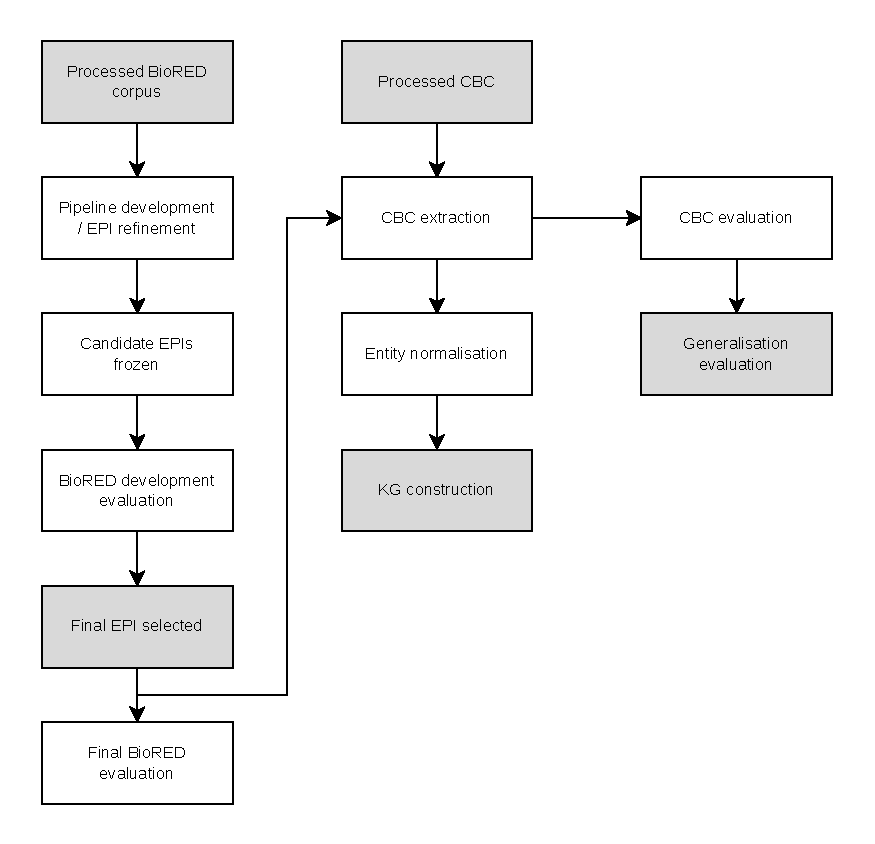
\includegraphics[width=\textwidth]{../img/system_architecture.pdf}
    \caption{System architecture and data flow, from prepared corpus input through extraction, normalisation, and \gls{kg} construction, to the three evaluation branches described in Section~\ref{sec:meth:evaluation}. Grey shading highlights key inputs, final stages, and outputs.}
    \label{fig:system_architecture}
\end{figure}

\section{Information Extraction Pipeline}
\label{sec:meth:info_extraction_pipeline}

\subsection{LLM Configuration}
\label{subsec:meth:llm_config}

\subsection{Prompt and Extraction Schema}
\label{subsec:meth:prompt_and_extraction_schema}

\subsection{Structured Output and Parsing}
\label{subsec:meth:structured_output_and_parsing}

\subsection{Entity Normalisation}
\label{subsec:meth:entity_normalisation}

\section{Pipeline Development}
\label{sec:meth:pipeline_development}

\subsection{Extraction Pipeline Iterations}
\label{subsec:meth:extraction_pipeline_iterations}

\subsection{Development and Model Selection}
\label{subsec:meth:development_and_model_selection}

\subsection{Final Pipeline}
\label{subsec:meth:final_pipeline}

\section{Contemporary Knowledge Graph Construction}
\label{sec:meth:contemporary_kg_construction}

\subsection{Contemporary Corpus Extraction}
\label{subsec:meth:contemporary_corpus_extraction}

\subsection{Graph Construction}
\label{subsec:meth:graph_construction}

\subsection{Ontology-Based Validation}
\label{subsec:meth:ontology_based_validation}

\section{Evaluation}
\label{sec:meth:evaluation}

\subsection{Entity Evaluation}
\label{subsec:meth:entity_evaluation}

\subsection{Relation Evaluation}
\label{subsec:meth:relation_evaluation}

\subsection{Generalisation Evaluation}
\label{subsec:meth:generalisation_evaluation}

\subsection{Knowledge Graph Evaluation}
\label{subsec:meth:knowledge_graph_evaluation}

\section{Cost Analysis}
\label{sec:meth:cost_analysis}
